% Lecture date: 05/06/2019, part one and two
% Authors: Ambuj Ojha, Kuixian Zhu, Yang Stelmach
% Time interval: entire class
\chapter{Self-Supervised Learning}

\section{Introduction and Why Self-supervised Learning}

The success story of computer vision can be viewed as the success story of supervision. For example, over the past decade, there has been continuous improvement in classification results on the ImageNet Challenge. 

Moreover, it has been shown that features from networks that are pre-trained on large datasets like ImageNet could be used for a variety of different downstream tasks. There is a general agreement that the 'recipe' for a computer vision supervised task is to:

\begin{itemize}
    \item Pre-train the model (usually a ConvNet) on a large supervised dataset
    \item Collect a dataset of supervised images
    \item Keep training the model
\end{itemize}

However, for a variety of data, such as video and medical images, it is hard to scale the labeling to the size of data we generate. Sadly, the labeled data that we are able to utilize is only an incredibly small portion of the data in our real world. Unlabelled internet images are several orders of magnitudes larger than labelled images. For instance, it would take 22 human years to label the remainder of ImageNet data. Thus, it is important for us to develop a 'self-automatic' process that can obtain labels from the data itself, which is the common definition of self-supervised learning.

One of the most successful examples of self-supervised learning is the representation learning in NLP. From  Word2vec (Mikolov et al.) to BERT (Devlin et al.), it has been shown that self-supervised learning can be helpful in getting high-quality sentence/word representations.

Indeed, self-supervised learning is helpful because it:

\begin{itemize}
    \item Helps us learn using observations and interactions
    \item Does not require exhaustive annotation of concepts
    \item Leverages multiple modalities or structures in the domain
\end{itemize}

\section{Self-supervised Learning in Computer Vision}

For computer vision, below three things are most popular:
\begin{itemize}
    \item Using images
    \item Using video
    \item Using video and sounds
\end{itemize}{}

\subsection{Using images}
Images always have an underlying spatial structure. This regularity is also the reason why convolutional network really works with images. 

\begin{itemize}
    
\item One of the first successful applications of self-supervised learning using images is in the task of finding the relative position of patches. The idea is to sample two patches in an image, for example - in the image of the cat in Fig.\ref{fig:1} one (blue patch) is the nose of the cat and the other (red patch) is on the eye of the cat. 

\begin{figure}[h!]
  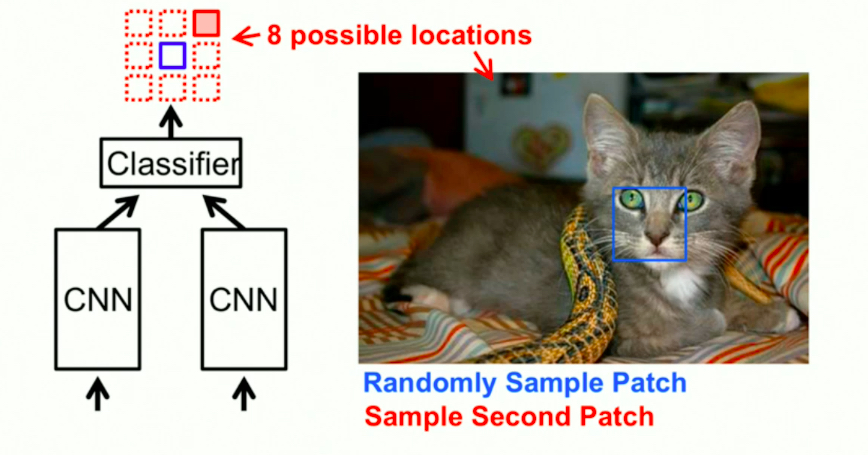
\includegraphics[width=\linewidth]{RelativePosition.jpg}
  \caption{Relative Position of patches}
  \label{fig:1}
\end{figure}

The first patch is fed in one CNN and the second patch is fed in another CNN. We then put a classifier on top to predict the relative spatial location of the two patches. Depending on where the blue patch is, we get 8 different classes (see Fig.\ref{fig:1} This is automatically generated supervision since we train the CNN to perform this task on a bunch of images without any human supervision.

In order for the network to be able to predict the relative position of patches, it needs to understand the spatial structure of the object. Essentially this task is training the network to encode spatial structure based on two glimpses.

In order to evaluate the representation, feature representation was computed for the network followed by computation of nearest neighbours for this feature representation. Essentially this tells us which patches this network thinks are similar and which patches are not similar. For any input, we see that the nearest neighbours computed by the relative position embedding retrieves patches which are very similar to the input. However the nearest neighbours computed by a randomly initialized CNN are not meaningful. Also comparing it with a model that was pre-trained on ImageNet also provides nice results as expected with strong supervision. This is a simple self-supervised learning task where by encoding different types of spatial structures, we learn a very powerful feature representation.

\item Another task is predicting colors at each pixel from a black and white image. Essentially it teaches the network to recognize objects in order to color them. 

\item One other interesting task is that given an image, if we block out a part of the image and train the network to reconstruct the blocked out part of the image. 

\item Another curious example of a task is predicting rotations in an image. Given an image, rotated in 4 different ways (either 90 deg, 180 deg, 270 deg or 0 deg), feed forward the image and ask the network to perform a four way classification to predict which particular rotation was applied to the image. Essentially just by doing this, the network learns to captures a very natural bias about the structure of the visual world.
\end{itemize}{}

\subsection{Evaluating self-supervision tasks}
Standard methodology for evaluation is treating self-supervised learning as a pre-training task. We have a bunch of images that is our pre-training data and we pre-train a CNN using either of the tasks discussed before (e.g. image colorization) and the CNN learns a visual representation. We can now fine-tune this representation on an end task where we have semantic supervision (e.g. image classification). One problem with this is that the fine-tuning step trains the full representation on the end task. So it tests both the initialization capabilities of the self-supervised pre-training as well as how good the representation is. In some way it conflates optimization with representational power.

